\documentclass{lkx_paper}

\title{Cosmological Constraints from \\Baryonic Acoustic Oscillations}
\date{April 2025}
\author{Lev Kruglyak}

\lkxbib{final-paper}

\usepackage{graphicx}
\usepackage{float}
\usepackage[skip=2pt]{caption}
\usepackage{titling}
\setlength{\droptitle}{-5em} 

\renewcommand{\d}{{\mathrm{d}}}
\renewcommand{\b}{{\mathrm{b}}}
\renewcommand{\c}{{\mathrm{c}}}
\newcommand{\bc}{{\mathrm{bc}}}
\newcommand{\K}{{\mathrm{K}}}
\newcommand{\m}{{\mathrm{m}}}
\newcommand{\DE}{{\mathrm{DE}}}
\newcommand{\MC}{{\mathrm{MC}}}
\newcommand{\eff}{{\mathrm{eff}}}
\newcommand{\CMB}{\mathrm{CMB}}

\newcommand{\LCDM}{$\Lambda\mathrm{CDM}$~}
\newcommand{\wwCDM}{{$w_0 w_a\mathrm{CDM}$~}}

\DeclareMathOperator{\diag}{{\operatorname{diag}}}

\newcommand{\MM}{{\mathcal{M}}}
\newcommand{\DD}{{\mathcal{D}}}
\newcommand{\UU}{{\mathcal{U}}}
\newcommand{\NN}{{\mathcal{N}}}
\newcommand{\LL}{{\mathcal{L}}}
\usepackage{bm}
\newcommand{\pms}{{\bm{\theta}}}
\newcommand{\Neff}{{N_\mathrm{eff}}}

\usepackage{siunitx}
\renewcommand{\si}[1]{\qty[per-mode = symbol]{#1}{}}
\providecommand{\Mpcsi}[1]{\qty{#1}{\mathrm{Mpc}}}
\providecommand{\eVsi}[1]{\qty{#1}{\mathrm{eV}}}
\providecommand{\Hsi}[1]{\qty{#1}{\km\,\s^{-1}\,\mathrm{Mpc}^{-1}}}

\begin{document}

In this paper, we use measurements of baryon acoustic oscillation (BAO) measurements by the Dark Energy Spectroscopic Instrument (DESI) to obtain constraints on cosmological parameters in the \LCDM model. This analysis has already been done in \cite{desicollaboration2025desidr2resultsii}, here we attempt to recreate some of the constraints obtained in that paper.

\subsection*{The \LCDM Model}
We begin with a brief review of the \LCDM model. The base geometry is the FLRW metric -- we assume further that it is flat.
Energy density in the model is thus split into five species: baryonic matter $\Omega_\b$, cold (i.e. non-relativistic) dark matter $\Omega_\c$, electromagnetic radiation $\Omega_\gamma$, curvature $\Omega_\K$, neutrinos $\Omega_\nu$, and dark energy $\Omega_\DE$. Note that the curvature energy density $\Omega_K=0$ is trivial, so we do not include it here. Baryonic and cold dark matter are grouped as $\Omega_\bc=\Omega_\b+\Omega_\c$, and non-relativistic matter including neutrinos is grouped as $\Omega_\m=\Omega_\bc+\Omega_\m$.
Using standard equation of state parameters for $\Omega_\bc$, $\Omega_\gamma$, and $\Omega_K$, we can write the time-dependent Hubble parameter as:
\begin{equation}
  \frac{H(z)}{H_0} = 
  \left[\Omega_\bc(1+z)^3 + \Omega_\gamma(1+z)^4+\Omega_\nu\frac{\rho_\nu(z)}{\rho_{\nu,0}} + \Omega_\DE \frac{\rho_\DE(z)}{\rho_{\DE,0}}\right]^{1/2}.
\end{equation}
The energy density of neutrinos begins scaling as $(1+z)^4$ at high redshifts and transitions to $(1+z)^3$. Throughout, we assume the existence of a single species of massive neutrino with mass $m_\nu = \eVsi{0.06}$ and $\Neff=3.044$. In the base \LCDM model, we assume that dark energy is constant over time, namely that $\rho_{\DE}(z)/\rho_{\DE,0}=1$. We remove this assumption later in the paper.

When performing Bayesian analysis on the \LCDM model, we sample along the six independent parameters of the model: $(\omega_\c, \omega_\b, \theta_*, \ln(10^{10}A_s), n_s, \tau)$. The first of these two parameters describe the ratios of cold dark matter and baryonic matter in the universe, i.e. $\omega_\c=\Omega_\c h^2$ and $\omega_\b = \Omega_\b h^2$ where $h=H_0/\Hsi{100}$. The next parameter, $\theta_*$ is the angular size of the sound horizon the surface of last scattering, i.e.
\begin{equation}
  \theta_* = \frac{r_s(z_*)}{D_A(z_*)}\quad\textrm{where}\quad
  r_s(z) = \int_z^\infty \frac{c_s(z')}{H(z')}\,dz'\quad\textrm{and}\quad D_A(z)=\frac{1}{1+z}\int_0^z\frac{c}{H(z')}\,dz'
\end{equation}
where $z_*\approx 1090$ and $c_s(z)$ is the speed of sound in the primordial photon-baryon fluid. To speed up computation, it is common to approximate $\theta_*$ by a parameter $\theta_\MC$ given by fitting formula in \cite{Lewis_2000}. The remaining parameter $\ln(10^{10} A_s), n_s,$ and $\tau$ are the amplitude and spectral index of the primordial scalar perturbations and the optical depth respectively. 

To perform Bayesian analysis with the CMB and DESI datasets, we use \texttt{Cobaya} \cite{Torrado_2021}, a general purpose Python program for exploring posterior distributions using Monte Carlo samplers. We use \texttt{CAMB} as the theoretical model backend for Cobaya analysis and use a Markov Chain Monte Carlo (MCMC) sampler with convergence criterion $R-1<0.01$ in the Gelman-Rubin statistic.

\subsection*{Exploring the CMB $H_0,\Omega_\m$ Degeneracy}

We begin by using the full CMB data from Planck 2018 to derive  

\begin{figure}[ht]
  \renewcommand{\arraystretch}{1.2}
  \centering
  \begin{tabular}{|c|c|c|c|c|c|c|}
    \hline
    parameter & $\omega_\c$ & $\omega_b$ & $100\theta_\MC$ & $\ln(10^{10} A_s)$ & $n_s$ & $\tau$\\
    \hline
    default & $\UU[0.001, 0.99]$ & $\UU[0.005, 0.1]$ &$\UU[0.5,10]$ &$\UU[1.61,3.91]$ &$\UU[0.8,1.2]$ & $\UU[0.01, 0.8]$  \\
    \hline
    BBN & $\NN(0.02218, 0.00055)$  &-&-&-&-&- \\
    \hline
  \end{tabular}
  \medskip
  \caption{Priors for $(\omega_\mathrm{c}, \omega_\mathrm{b}, 100\theta_{\mathrm{MC}}, \ln(10^{10}A_s), n_s, \tau)$.}
\end{figure}


\begin{figure}[ht]
  \centering
  \[
    \begin{aligned}
      (\theta_*, \omega_\b,&\; \omega_\c)_{\CMB} \quad\sim\quad\\ 
                                              &\NN\left(
\begin{bmatrix}
0.01041009 \\
0.02219065 \\
0.11969417
\end{bmatrix},
\begin{bmatrix}
5.10125839\times10^{-12} & 6.40183333\times10^{-11} & -6.09287501\times10^{-10} \\
6.40183333\times10^{-11} & 1.62733275\times10^{-8}  & -6.32279490\times10^{-8}  \\
-6.09287501\times10^{-10} & -6.32279490\times10^{-8} & 1.08987992\times10^{-6}
\end{bmatrix}\right)
    \end{aligned}
\]
  \caption{Derived CMB prior on $(\theta_*, \omega_\b, \omega_\c)$.}
\end{figure}

\subsection*{Baryonic Acoustic Oscillations}

  % thetastar:
  %   prior: {dist: norm, loc: 0.0104110, scale: 0.0000053}



When performing Bayesian analysis with the \LCDM model, 

These parameters are passed to \texttt{CAMB} \cite{Lewis:1999bs}

\subsection*{Results}


\begin{figure}[H]
  \centering
  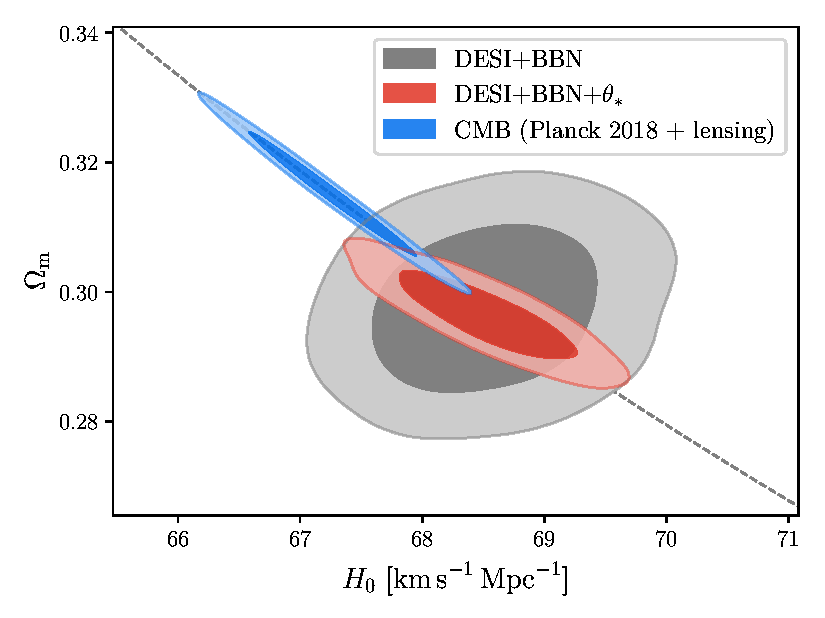
\includegraphics[scale=0.8]{figures/H0-omegam.pdf}
  \caption{}
\end{figure}

\begin{figure}[H]
  \centering
  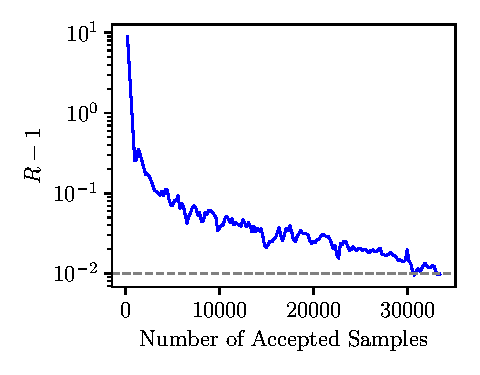
\includegraphics{figures/CMB-R-1.pdf}
  \caption{}
\end{figure}

\subsection*{The Behavior of Dark Energy}

In the base \LCDM model, dark energy is assumed to be constant, i.e. $\rho_\DE(z)/\rho_{\DE,0}=1$. However, it is common to extend the theory by allowing dark energy to have a varying equation of state parameter. The usual parametrization is:
\begin{equation}
w(z)=w_0+w_a(1-a)\quad\implies\quad
  \frac{\rho_\DE(z)}{\rho_{\DE,0}} = a^{3(1+w_0+w_a)}e^{-3w_a(1-a)}.
\end{equation}
This model is known as the \wwCDM model.

\end{document}
